\chapter{Data}
\label{chap:three}

Compared to traditional financial data cryptocurrency data tend to be easier
to obtain. However, many data providers have already identified the bussiness 
potential of selling advanced data and have started to monetize them. Since some
websites monetize only their APIs we could obtain data from 
multiple sources and merge them to get to our desired number of features. We have
desired to use as many relevant variables as possible and we build on
an existing research in the field.
Our dataset can be split into 2 main categories and 4 subcategories.
We utilize the data that describe the overall market trends in the traditional
sense. These data were mostly obtained from \textbf{\href{https://fred.stlouisfed.org/}{Federal Reserve Bank of St. Louis}}
and from the 
\textbf{\href{https://finance.yahoo.com/markets/}{Yahoo Finance}} API.
To balance fundamental indicators with speculative side we used \textbf{\href{https://trends.google.com/trends/}{Google Trends}}
and \textbf{\href{https://pageviews.wmcloud.org/}{Wikipedia Page Views}} 
that act as a proxy for market attention about cryptocurrencies in general 
and should help us to model the market hype periods. These explanatory
variables are then used to forecast the price or returns of the specific cryptocurrency
of interest lagged back in time.

\begin{figure}[!h]
    \centering
    \caption{Dataset Variables Overview}
        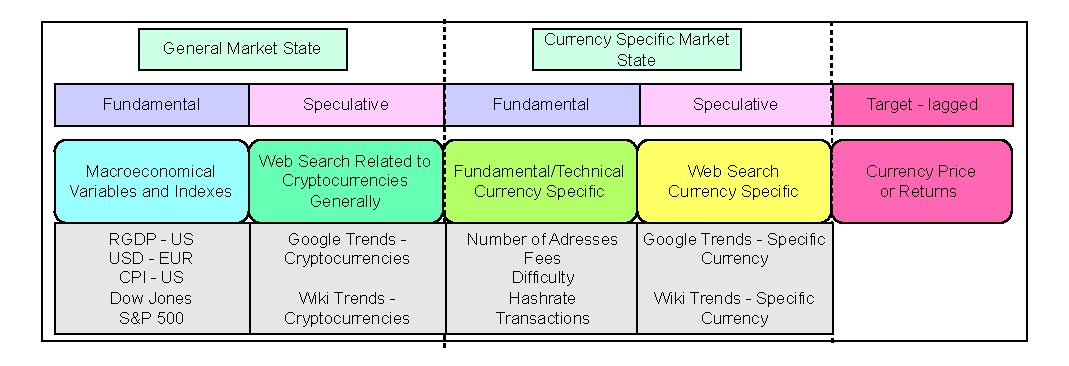
\includegraphics[width=1\textwidth]{Figures/dataset_description.drawio.pdf}
    \label{fig:dataset_description}
\end{figure}


The data were collected between December 2023 to February 2024 varying 
based on
the different sources but they are further shortened to utilize the most
overlapping region between data sources for each unique cryptocurrency.
This results in a time series from 17.9.2014 to 1.11.2022 for Bitcoin, 4.2.2016
to 27.7.2022 for Ethereum ensuring that the end of the series is 
before the change to proof-of-stake algorithm and series from 17.9.2014 to 1.11.2022
for Litecoin. The shifted versions of the datasets are of variable length based
on the forecasting horizon. 
\section{Cryptocurrency Specific Technical Data}

Despite the fact, that we have framed this data as fundamental/technical 
we should acknowledge that fundamental in our case stands far from its 
traditional meaning. They are fundamental in a way that they 
are the typical data researchers and practitioners employ to model cryptocurrencies
and that they objectively describe the system.
However, as the fundamental factor is very limited in this case it only makes sense
for the typical variables such as capitalization, volatility, hashrate and others.
But we also used a lot of technical variables that are derived from these fundamental
variables or the price itself. These help to identify trends in certain 
variables from pure mathematical transformation of the original series. 
All of these data were collected from \textbf{\href{https://coinmetrics.io/}{coinmetrics.io}}
and further processed by our pipeline.


We incorporate many variables describing specific technical characteristics of the network. Starting with number of active addresses
which acts as a measure of user activity on a particular day that is a cruical parameter potentially capturing the strength of 
bull or bear market behaviour. However, it does not reflect the direction itself. The difficulty of the network is
adjusted dynamically to counteract the changes in the mining power and thus act as a proxy for current mining power of the network or the current efforts of the miners. 
The size of the block is another characteristic of the network describing the size of the block (in bytes) and has been steadily increasing overtime
with significant fluctuation that depend on many other changes in the network. Hashrate is a measure of how
fast do the miners solve the hash for one block. In the long term the mean hashrate should be proportional to the difficulty at least that is how the 
\ac{BTC} protocol was designed however there are some fluctuation in the short term as the difficulty is adjusted every 2016 blocks 
to match the average hashrate over that period.


Other variables focus on the economics of the currency and model the market behaviour not the network itself. 
Beginning with traditional market signals such as capitalization indicating the overall price of all coins and volatility of returns 
as a standart deviation of log-returns. Furthermore, we employ many other variables about the price of fees 
provided by the users, revenues of the miners, distribution of wealth in the network and the number of transactions for that interval.


For the full description of the variables for \ac{BTC} please refer to the Appendix~\ref{app:var_desc}.


The datasets for Ethereum and Litecoin look similar with the exception of a few variables missing,
look at (\ref{ethereum:missing}, \ref{litecoin:missing}):

\begin{figure}[!htbp]
    \begin{center}
    \caption{Ethereum missing variables}\label{ethereum:missing}
    \begin{boxeditemize}
        \item \textit{Hash rate, mean, 30d}
        \item \textit{Supply, Miner, held by all mining entities, USD}
        \item \textit{Block, weight, mean}
    \end{boxeditemize}
    \end{center}
    \end{figure}

    \begin{figure}[!htbp]
        \begin{center}
        \caption{Litecoin missing variables}\label{litecoin:missing}
        \begin{boxeditemize}
            \item \textit{Hash rate, mean, 30d}
            \item \textit{Supply, Miner, held by all mining entities, USD}
            \item \textit{Flow, in, to exchanges, USD}
            \item \textit{Flow, out, from exchanges, USD}
            \item \textit{Revenue, per hash unit, USD}
        \end{boxeditemize}
        \end{center}
        \end{figure}


\section{Macroeconomical Data}

As the macroeconomical condition is a cruical factor for investor behaviour 
we decided to include relevant variables that might deliver valuable
insights. We utilize five macroeconomical indicators that affect invesment choices.
Real Gross Domestic product of the United States represents the overall
growth trend of the largest economy in the world with closely related real
gross domestic product per capita telling more about individual resouces which
gives a more complex picture of the state of the US economy despite the 
fact that americans are not the main cryptocurrency investors by nation.
Furthermore we incorporate Consumer Price Index in the United States that
acts as an inflationary measure to capture the spurious correlation between 
prices of USD and BTC-USD exchange rate. M2 base acts as a measure
of dollar liquidity in the circulation. Lastly, the USD-EUR exchange rate
can be thought of as a market state information or its returns as an 
opportunity costs for potential investors. To further adress the problem of spurious
correlation and add the information about growth of other markets we include
various closing prices and other measures of the stock market and other 
investment opportunities. 


Following is the full description of the macroeconomical
variables used:

\begin{itemize}
    \item \textit{Close\_DJI} - Dow Jones Industrial Average
    \item \textit{Close\_GSPC} - S\&P 500
    \item \textit{Close\_GC=F} - Gold Futures
    \item \textit{Close\_VIX} - CBOE Volatility Index
    \item \textit{Close\_IXIC} - NASDAQ Composite
    \item \textit{Close\_SMH} - VanEck Semiconductor ETF
    \item \textit{Close\_VGT} - Vanguard Information Technology Index Fund
    \item \textit{Close\_XSD} - SPDR S\&P Semiconductor ETF
    \item \textit{Close\_IYW} - iShares U.S. Technology ETF
    \item \textit{Close\_FTEC} - Fidelity MSCI Information Technology Index ETF
    \item \textit{Close\_IGV} - iShares Expanded Tech-Software Sector ETF
    \item \textit{Close\_QQQ} - Invesco QQQ Trust
    \item \textit{RGDP\_US} - Real Gross Domestic Product of the United States
    \item \textit{RGDP\_PC\_US} - Real Gross Domestic Product per capita 
    of the United States
    \item \textit{CPI\_US} - Consumer Price Index: All Items: Total for United States
    \item \textit{M2\_US} - M2 Base US
    \item \textit{USD\_EUR\_rate} - U.S. Dollars to Euro Spot Exchange Rate
\end{itemize}


\section{Web Search Data}

As mentioned earlier following many other researchers we aimed to 
obtain a proxy for the market
attention. We specifically used \textbf{\href{https://pageviews.wmcloud.org/}{Wikipedia Page Views}}
to get the page views for Wikipedia pages: Bitcoin, Ethereum, Litecoin and 
Cryptocurrency and use them respectively for each coin dataset combining 
the overall Cryptocurrency views with the specific currency. Similarly we 
hoped to obtain similar data from 
\textbf{\href{https://trends.google.com/trends/}{Google Trends}} but they
turned out to be quite cumbersome to use. As \cite{West2020a} mentioned 
there are three main obstacles when using Google Trends. Firstly, the scale
is always normalized into the range 0-100 based on the selected region and time.
Secondly, this implicitly means that the results are rounded to integers and thus 
loosing a lot of precision. Lastly, there is a limit of 5 queries that you can 
use at a time. This not only means that you cannot compare more search terms 
but it also means that when there are over five variations how the term might
be searched for one cannot do that effectively. Another problem, 
that we faced is that the data can be obtained only in weekly granularity
for longer periods and thus needs to be interpolated to daily which 
most likely sacrifices a lot of interesting dynamics on the daily level which
is significant regarding the volatility of cryptocurrencies. 
These reasons, except the weekly sampling frequency, were solved in 
the \textbf{\href{https://github.com/epfl-dlab/GoogleTrendsAnchorBank}{g-tab}}
Python library, created by \cite{West2020a}, which uses a 
two step query sampling process that 
estimates the searches on a universally common scale with floating precision and allows 
us to use as many word formulation as needed. We would then sum the popularity
for each word formulation that is related to the same thing. We acknowledge
that there is a risk that we ommited some word formulations but hopefully
we covered all the significant ones.


Following is the list of the variables from this section and their word forms
for Google Trends:
https://cs.wikipedia.org/wiki/Bitcoin
\begin{itemize}
    \item \textit{Wiki\_btc\_search} - Wiki pageviews for \textbf{\href{https://cs.wikipedia.org/wiki/Bitcoin}{Bitcoin}}
    \item \textit{Wiki\_eth\_search} - Wiki pageviews for \textbf{\href{https://cs.wikipedia.org/wiki/Ethereum}{Ethereum}}
    \item \textit{Wiki\_ltc\_search} - Wiki pageviews for \textbf{\href{https://cs.wikipedia.org/wiki/Litecoin}{Litecoin}}
    \item \textit{Wiki\_crypto\_search} - Wiki pageviews for \textbf{\href{https://en.wikipedia.org/wiki/Cryptocurrency}{Cryptocurrency}}
    \item \textit{Google\_btc\_search} - Google Trends summed from terms: \textit{Bitcoin, bitcoin, BTC}
    \item \textit{Google\_eth\_search} - Google Trends summed from terms: \textit{Ethereum, ethereum, ether, ETH}
    \item \textit{Google\_ltc\_search} - Google Trends summed from terms: \textit{Litecoin, litecoin, LTC}
    \item \textit{Google\_crypto\_search} - Google Trends summed from terms: \textit{Cryptocurrency, cryptocurrency, Cryptocurrencies, cryptocurrencies, crypto, Crypto}
\end{itemize}


\section{Preprocessing}


Forecasting from historical data comes with many identified challenges. These
were especially pronounced in our case as we incorporate data from many
different sources with different sampling frequencies. Despite the fact
that our focus is on forecasting daily price and returns we use data
that come in weekly and monthly frequencies. We suggest two general concerns 
with such data. As we are using historical explanatory variables
to predict a response variable in the future we need to ensure that our
explanatory variables are already published at the time of forecasting and not
use data from the future. We implement forward filling after the data is resampled
to daily frequencies as a remedy. Especially for the macroeconomical data
we implicitly match those indicators to future dates that they do not trully
corespond to. Concretely, the Consumer Price Index for January is published at the 
beginning of February but as we forward fill this variable the Consumer Price Index
from January will actually be in February. This ensures that when we are 
forecasting with a 10 day horizon at the beginning of February we only use
data that was present at that time. The second concern is the fact 
that there is a lot of lost signal during those interpolated periods 
and the daily dynamics are not incorporated in the model. Unfortunately,
this is the nature of economic research as especially the 
macroeconomical indicators come typically in such sampling frequencies.
As already suggested these preprocessing steps were applied to the macroeconomical
indicators, Google Trends that come in weekly frequency and for 
ETFs and indexes that are not traded on the weekends, see Figure~\ref{fig:dataset_interpolation}.

\begin{figure}[!h]
    \centering
    \caption{Dataset Feature Interpolation}
        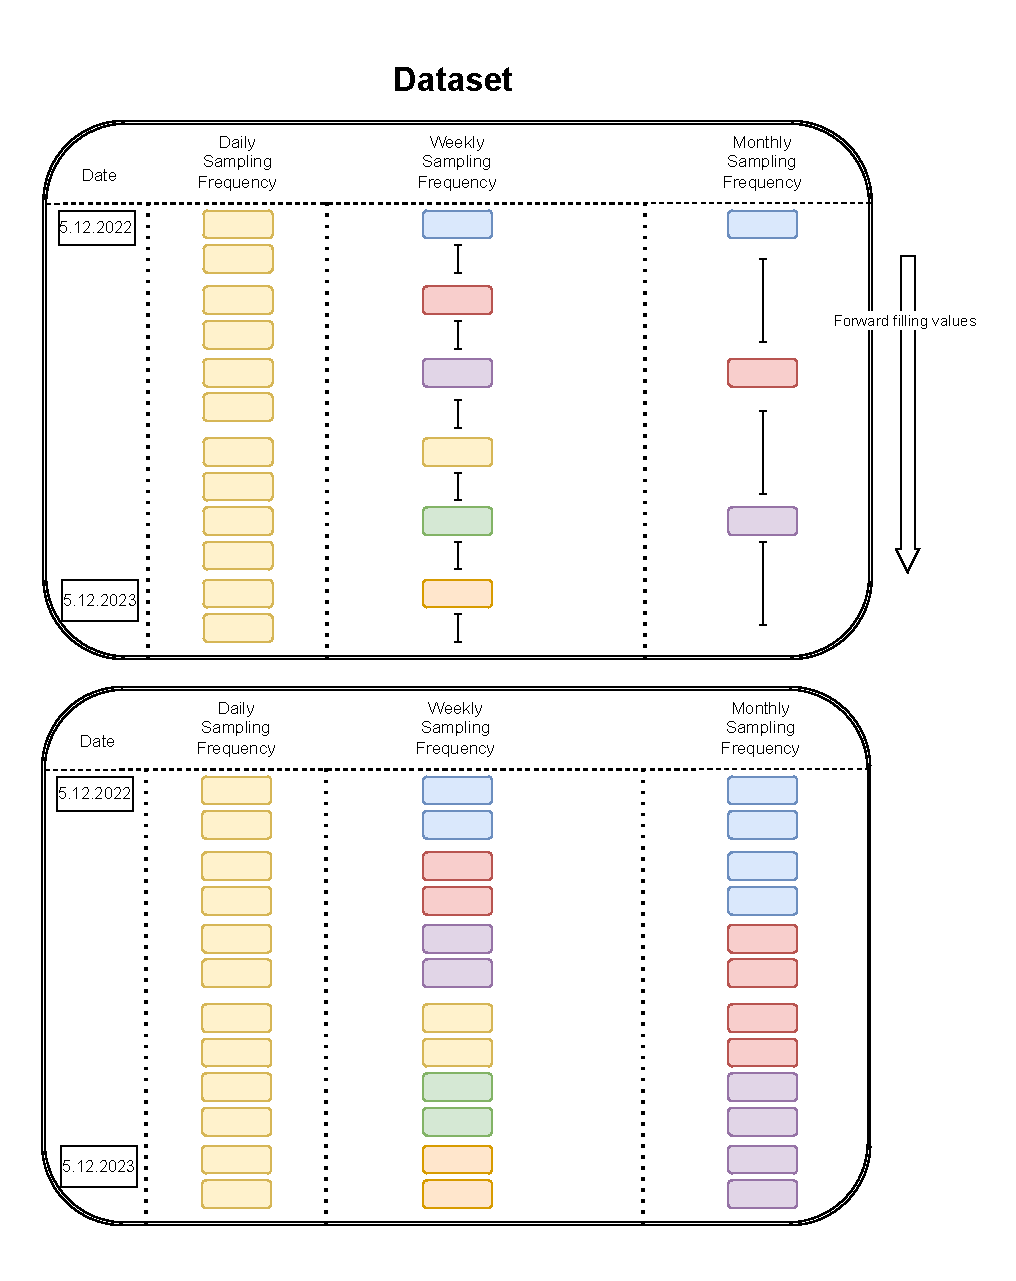
\includegraphics[width=1\textwidth]{Figures/data_interpolation.drawio.pdf}
    \label{fig:dataset_interpolation}
\end{figure}

As some of the variables are missing at the beginning of the time frame there
is no clear solution how to impute them without leaking the future distribution.
Even though we could say that this rule might be violated on the training set
but we opted for a different approach.
We start by visually inspecting the structure of the missing values and 
set the start of the series as such that "almost all" variables are already 
being collected. The aim is to keep as much data as possible but avoid
having a lot of data points at the beginning with different distribution changed 
by imputation. After that we fill the data that is missing only at the start with
zeros in order to avoid imputing future data. There is also a second reason
as generaly these variables are increasing and thus imputing zeros makes 
even mathematical sense. Especially for data like Googe Trends or Wikipedia
Pageviews this is a reasonable imputation. Finally we cut the 
\ac{ETH} series at the switch to proof-of-stake as this completely
changes the modeling perspective and we merge all the data
from different sources on the date column.


The most cruical step is the transformation of this dataset into a supervised
learning problem. We will proceed with the example of BTC price, however
the same will hold for other coins and returns forecasting. We employ
forecasting with 1, 5 and 10 day horizon $h$. We denote the number 
of observations $\mathbf{x_{i}}$
as $n$ and the number of features $j$ as $k$.

\begin{equation}\label{eq:horizon}
    h \in \{1,5,10\}
\end{equation}
\begin{equation}\label{eq:features}
    j \in \{1,...,k\}
\end{equation}
\begin{equation}\label{eq:observations}
    i \in \{1,...,n\}
\end{equation}

We start by denoting
the original dataset $\mathbf{X} \in \mathbb{R}^{n \times k}$.
Now assuming $\mathbf{X_{:,k}} = [\mathbf{x}_{1k},...,\mathbf{x}_{nk}]$ 
is the \ac{BTC} price feature vector we shift it
back in time by $h$ and drop the data without corresponding counterpart. 
Concretely, we drop all 
$\mathbf{X_{n-h:n,1:k-1}}$ and $\mathbf{X_{1:h,k}}$.
With this technique we always sacrifice $2h$ observations from the original dataset.
If we further split the dataset into the explanatory and target features
and reset the indexation such that we denote $m = n-2h$
we end up with the following matrices where the target matrix Y is essentially
only a vector where $y^\top = \mathbf{X_{:,k}}$, see Figure~\ref{fig:dataset_shift}.

\begin{figure}[!h]
    \centering
    \caption{Dataset Shifting for Supervised Learning}
        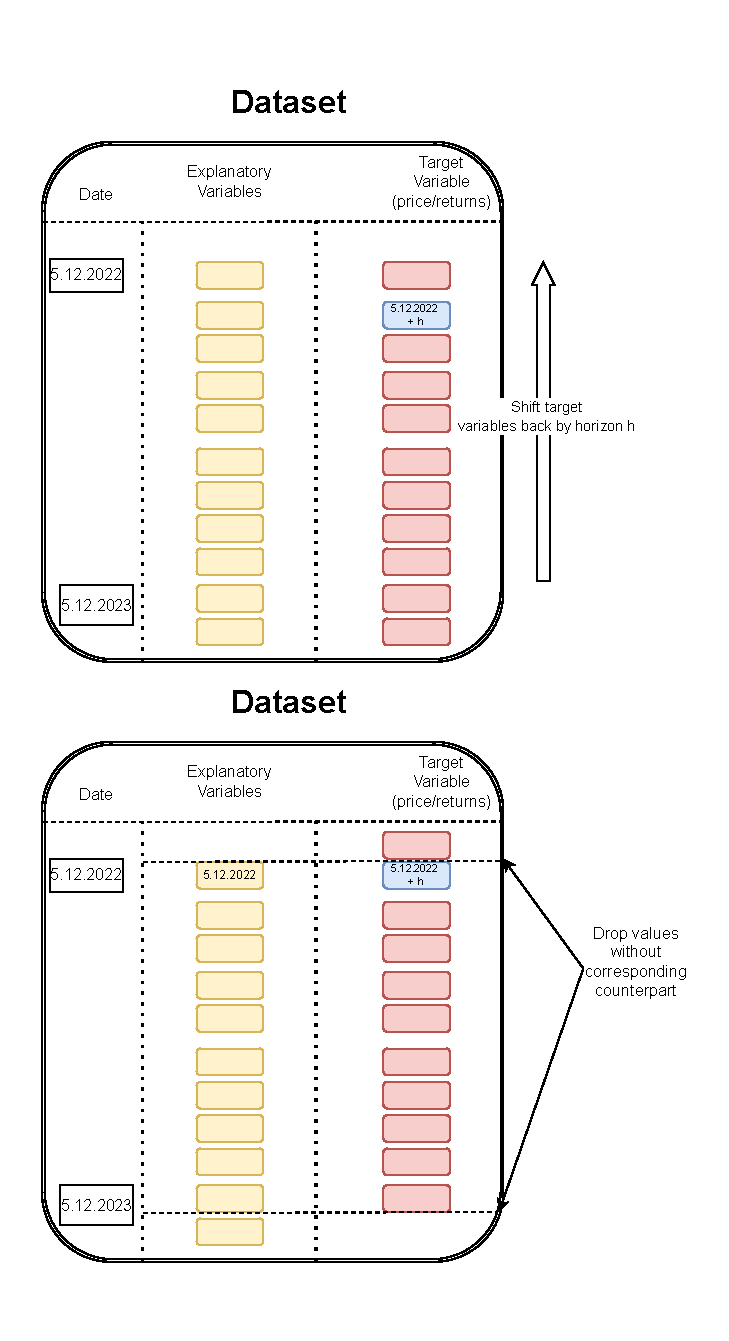
\includegraphics[width=1\textwidth]{Figures/data_shift.drawio.pdf}
    \label{fig:dataset_shift}
\end{figure}

\begin{equation}\label{eq:explanatory}
    \mathbf{X} \in \mathbb{R}^{m \times {k-1}} = 
    \begin{pmatrix}
        x_{11} & x_{12} & \dots  & x_{1k-1} \\
        x_{21} & x_{22} & \dots  & x_{2k-1} \\
        \vdots & \vdots & \ddots & \vdots \\
        x_{m1} & x_{m2} & \dots  & x_{mk-1}
    \end{pmatrix}
\end{equation}

\begin{equation}\label{eq:target}
    \mathbf{Y} \in \mathbb{R}^{m \times 1} = \mathbf{y^\top} = 
\begin{pmatrix}
    y_{1}\\
    y_{2}\\
    \vdots  \\
    y_{m} 
\end{pmatrix}
\end{equation}
We can now observe that modeling $y_i$ as a function of
explanatory variables $x_{i}$ is a forecasting with horizon $h$ into the future.
Where we essentially try to estimate the function $f_{foreacast}$.
\begin{equation}\label{eq:model_simple}
    y_i = f_{forecast}(\mathbf{x_{i}})
\end{equation}

The final preprocessing step is specific to the \ac{LSTM} network which is
a type of architecture that requires the input to be of 
the shape (num timesteps, num features).
This means that it can use for example 10 day history for each variable
and forecast the target variable. This is a really strong feature and 
makes it a viable option for our usecase. In order to use it, the input dataset
has to be reshaped in such a way that for observation $\mathbf{x_{i}}$ 
concatenates values from $\mathbf{x_{i}}$ 
up to $\mathbf{x_{i-lag}}$, see Figure~\ref{fig:dataset_lstm_reshape}


\begin{equation}\label{eq:lstm_reshape}
    \mathbf{X_{i,:}} = [[{x}_{i1},...,{x}_{ik}],
    [{x}_{i-11},...,{x}_{i-1k}],
    [{x}_{i-lag1},...,{x}_{i-lagk}],...]
\end{equation}

\begin{figure}[!h]
    \centering
    \caption{LSTM Reshaping}
        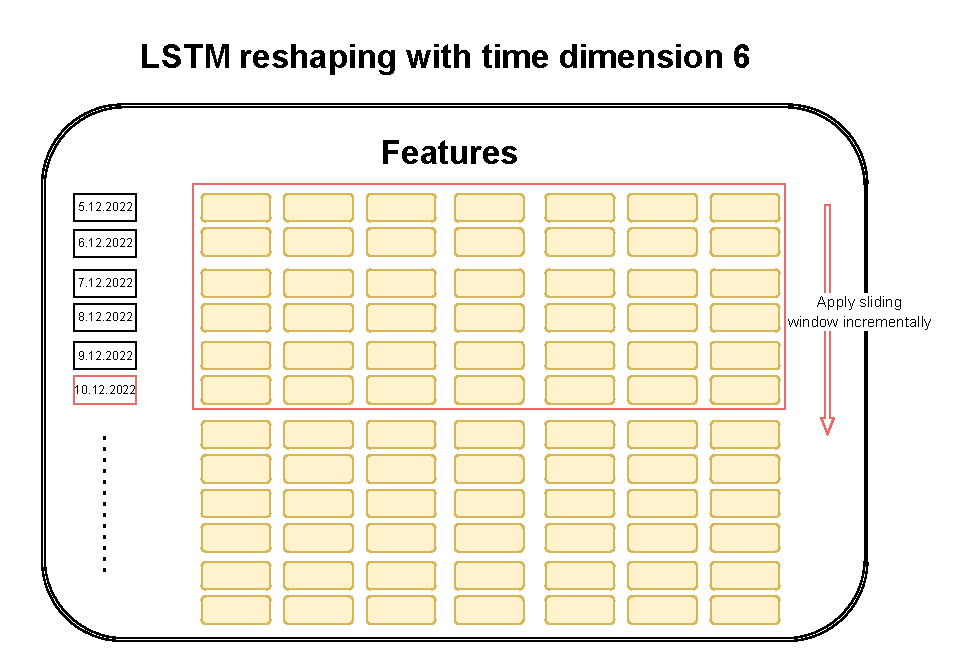
\includegraphics[width=1\textwidth]{Figures/LSTM_reshaping.drawio.pdf}
    \label{fig:dataset_lstm_reshape}
\end{figure}